\documentclass{article}

\usepackage[dutch]{babel}
\usepackage[margin=3cm]{geometry}
\usepackage{graphicx}
\usepackage{float}
\usepackage{caption}
\usepackage{hyperref}
\usepackage{amsmath}
\usepackage{wrapfig}
\usepackage[parfill]{parskip}

% fonts
\usepackage[T1]{fontenc}
\usepackage{helvet}
\renewcommand{\familydefault}{\sfdefault}

\graphicspath{{img/}}
 
\newcommand{\bold}[1]{\textbf{#1}}

%Define the listing package
\usepackage{listings} %code highlighter
\usepackage{upquote}
\usepackage{color} %use color
\definecolor{mygreen}{rgb}{0,0.6,0}
\definecolor{mygray}{rgb}{0.5,0.5,0.5}
\definecolor{mymauve}{rgb}{0.58,0,0.82}

\begin{document}

\begin{titlepage}
    \author{Tuur Vanhoutte}
    \title{IoT Cloud}
\end{titlepage}

\pagenumbering{gobble}
\maketitle
\newpage
\tableofcontents
\newpage

\pagenumbering{arabic}

\section{Cloud computing}

= the practice of using a network of remote servers hosted on the Internet to store, manage, and process data, rather than a local server or a personal computer.

\subsection{Enkele eigenschappen}
\begin{itemize}
    \item Geen eigen hardware (we kopen niets aan)
    \item Ongelimiteerde computing power
    \item Ongelimiteerde storage capaciteit
    \item Scaling up and down op aanvraag of
    automatisch
    \item Scaling in en out op aanvraag of
    automatisch
    \item Geografische spreiding
    \item Pay what you use
\end{itemize}

\begin{figure}[H]
    \centering
    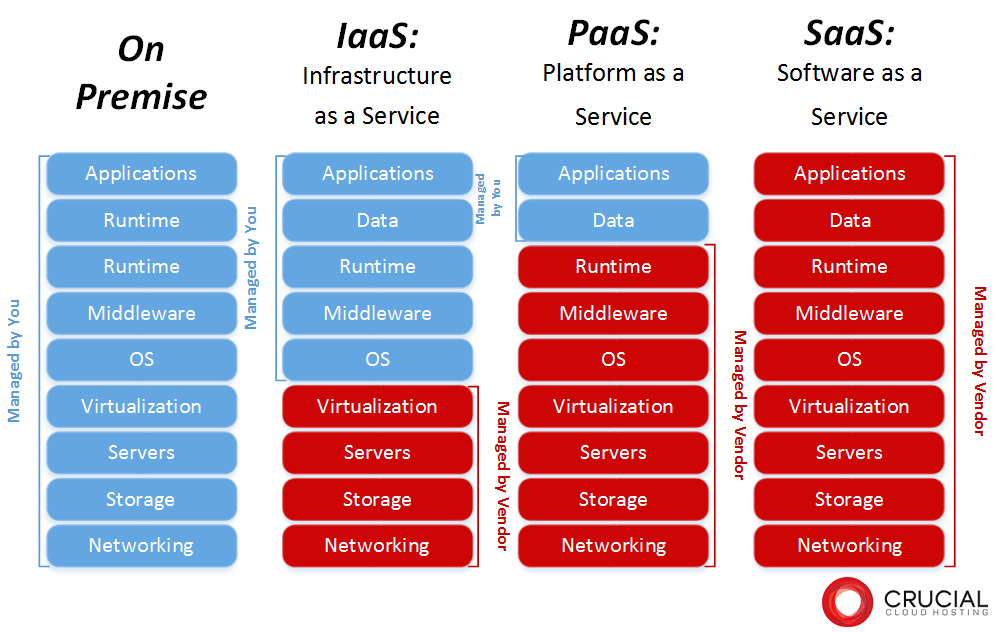
\includegraphics[width=0.7\textwidth]{cloud-hosting.png}
    \caption{}
\end{figure}


\subsection{On premise (eigen servers)}

\begin{itemize}
    \item 
    \item IT Afdeling is verantwoordelijk voor ALLES
    \item Back-up \& recovery
    \item Aankoop hardware
    \item Scaling...
    \item Meeste vrijheid om te werken
    \item Soms investeren in hardware die je maar beperkt aantal dagen nodig hebt
    \item Vb: webshop en kerstperiode
    \item Soms verplicht door wetgeving
    \item Medische data
    \item Financial data
    \item Gebrek aan vertrouwen bij public cloud provider (cfr NSA)
\end{itemize}

\subsection{Hybrid Cloud (On Premise \& Cloud)}
Makes use of existing in-house infrastructure and Netplan cloud services to provide the best of both worlds.

\begin{itemize}
    \item Eigen datacenter koppelen aan cloud omgeving
    \item Bepaalde diensten draaien in cloud omgeving andere in eigen datacenter
    \item Zware load laten uitvoeren op de cloud
    \item Bepaalde data mag NIET in cloud opgeslagen worden vb: medical
    \item Kan ook gebruikt worden in back-up scenario’s
\end{itemize}

\subsection{IaaS: Infrastructure as a Service}

\begin{itemize}
    \item Geen eigen hardware kopen
    \item We huren virtual machines in Cloud omgeving
    \item Systeem beheerder moet zelf server configureren en beveiligen en updaten
    \item Veel flexibiliteit naar software installatie toe
    \item Zeer veel vrijheid maar ook verantwoordelijkheid
    \item Je moet zelf scaling doen (soms auto scaling mogelijk)
    \item Veel gebruik voor migratie bestaande On Premise naar cloud
\end{itemize}

\subsubsection{Voorbeelden}
\begin{itemize}
    \item Amazon Web Services (AWS)
    \item Microsoft Azure
    \item IBM Bluemix
    \item Google Cloud platform
\end{itemize}

\subsection{PaaS: Platform as a Service}

\begin{itemize}
    \item Geen systeembeheerder nodig
    \item Ontwikkelaar maakt applicatie en "plaatst" deze op Cloud platform
    \item We moeten ons geen zorgen maken in servers, hosting, back-ups, scaling,... het platform zal dit voor ons beheren
    \item Zeer veel flexibiliteit
\end{itemize}

We zullen vooral dit gebruiken in IoT Cloud module.

\subsubsection{Talen}
\begin{itemize}
    \item ASP.NET Core
    \item NodeJS
    \item Python
    \item Java
    \item PHP
\end{itemize}

\subsubsection{Voorbeelden}
\begin{itemize}
    \item Amazon Web Services (AWS)
    \item Microsoft Azure
    \item IBM Bluemix
    \item Google Cloud platform
    \item Heroku
\end{itemize}

\subsection{SaaS}
\begin{itemize}
    \item Software draait meestal niet lokaal (uitzondering Adobe \& Office)
    \item We betalen per maand/gebruiker
    \item Flexibele abonnementen, snel op te zetten
    \item We moeten geen rekening houden met back-ups en uptime
\end{itemize}

\subsubsection{Voorbeelden}
\begin{itemize}
    \item salesforce
    \item Office 365
    \item Dropbox, OneDrive, Google Drive, iCloud
    \item Gmail
    \item Adobe Creative Cloud
\end{itemize}

\subsection{Belangrijkste vendors}
\begin{itemize}
    \item Amazon Web Services
    \item Microsoft Azure
    \item Google Cloud Platform
\end{itemize}

\begin{figure}[H]
    \centering
    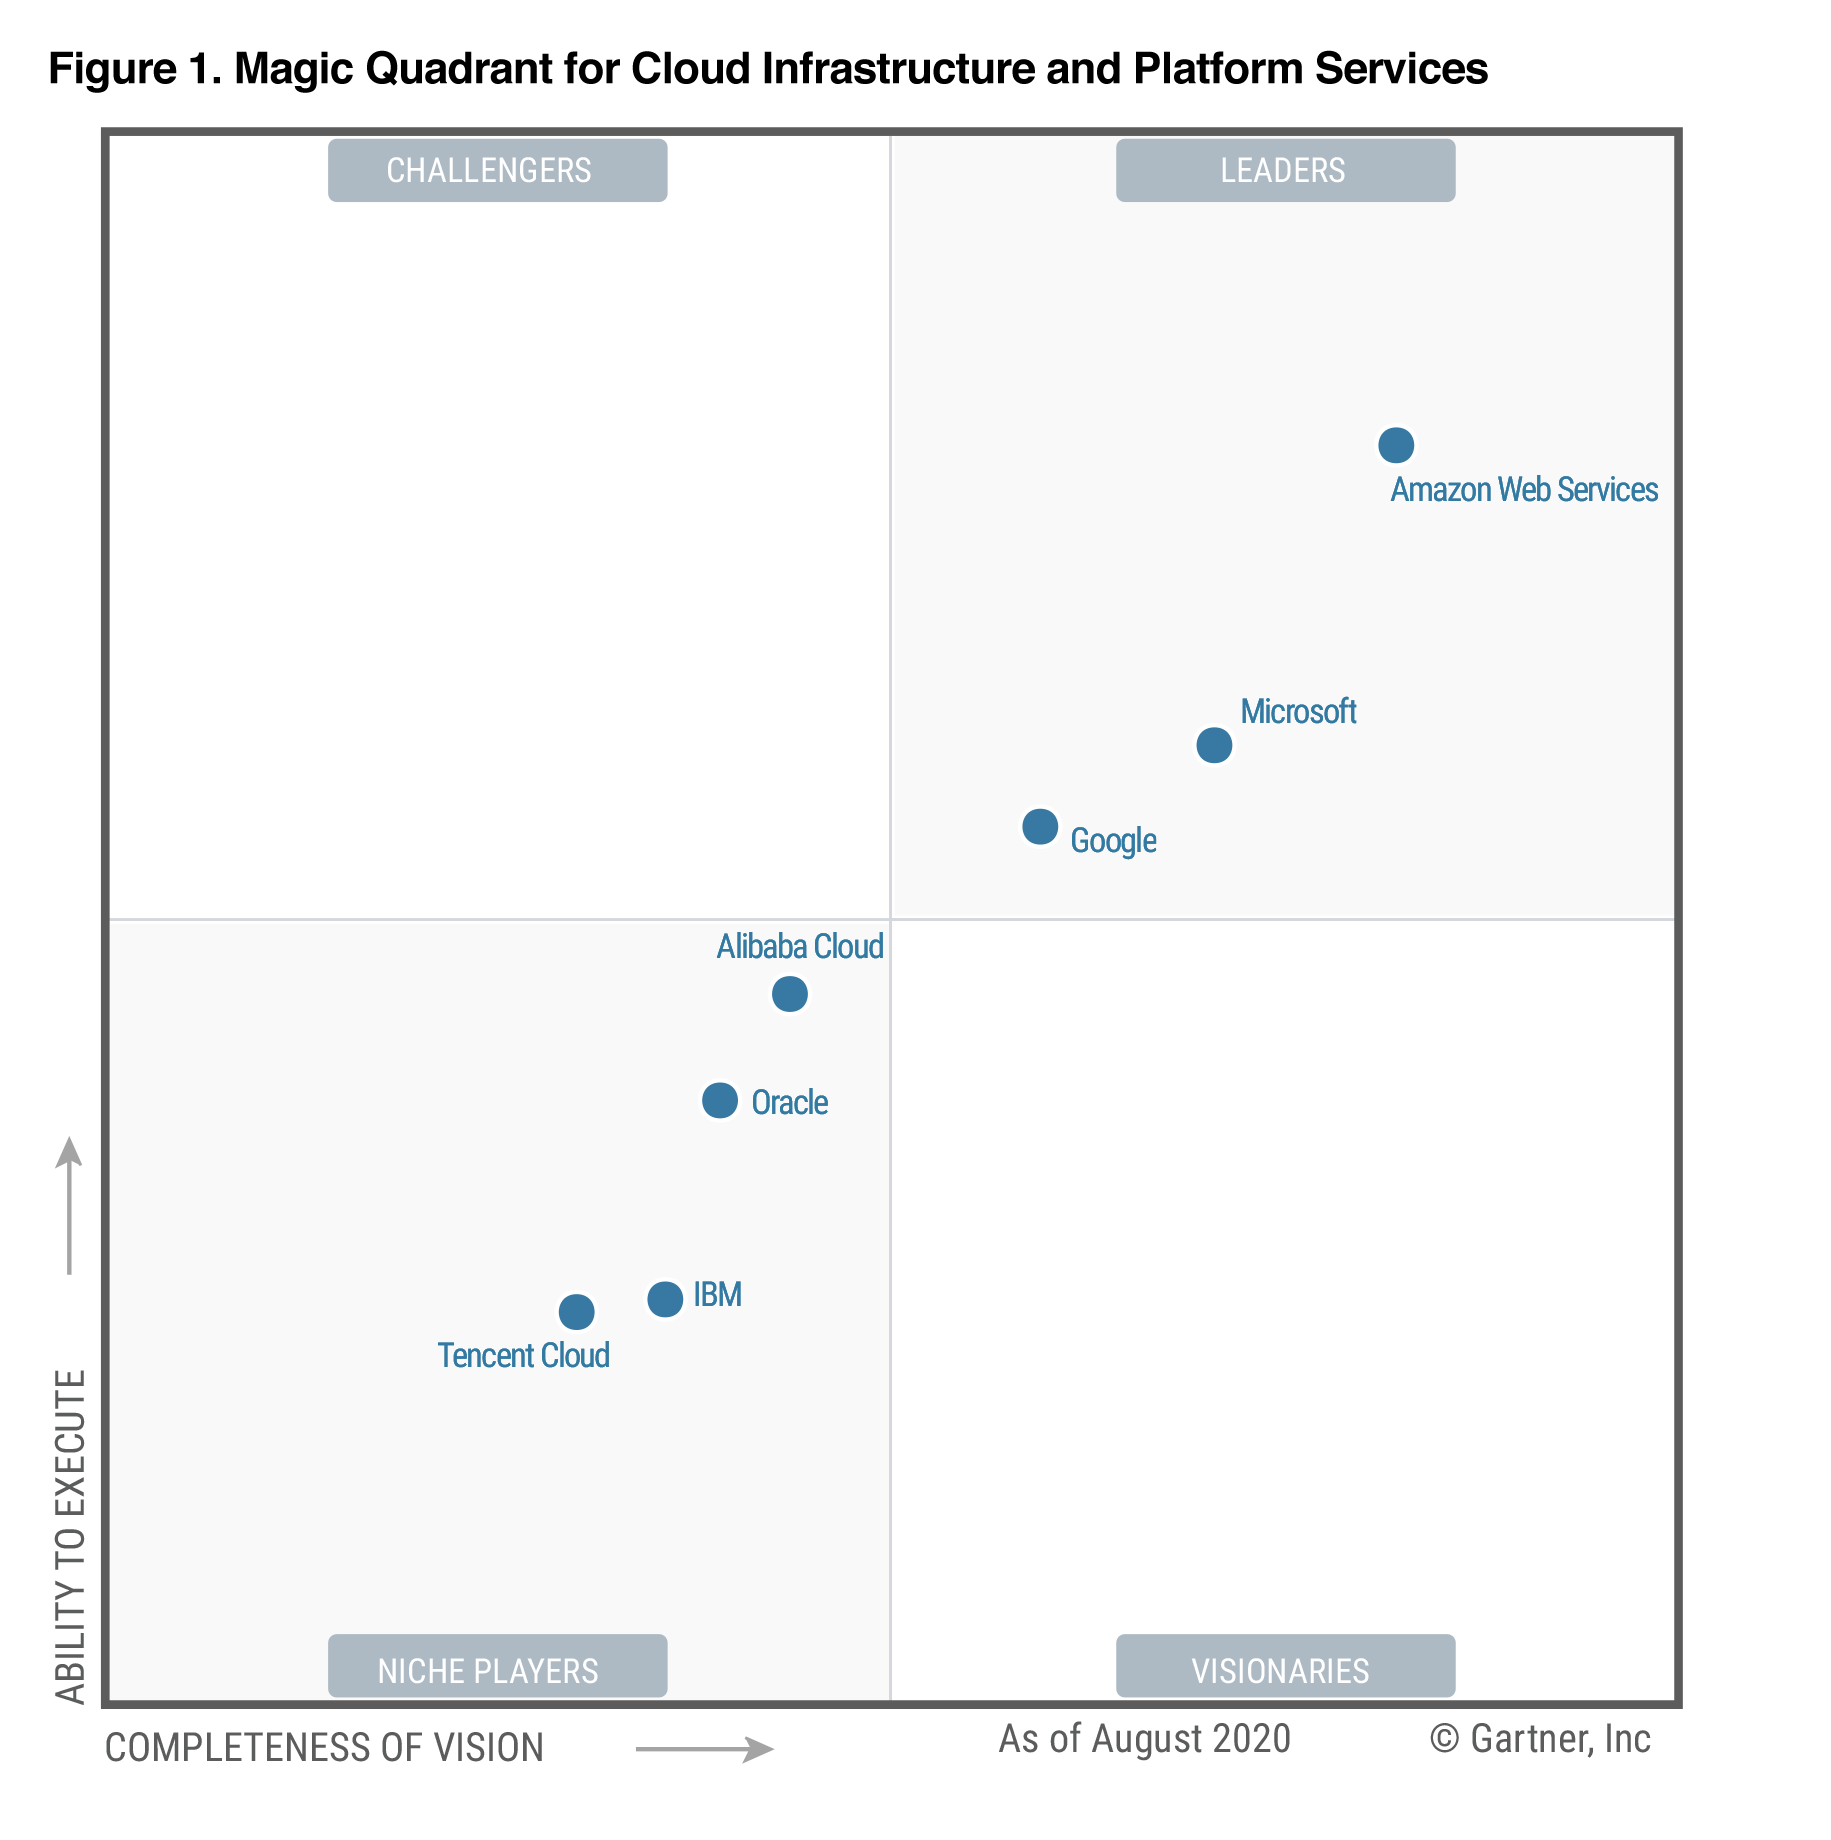
\includegraphics[width=0.5\textwidth]{magic-quadrant.png}
    \caption{}
\end{figure}



\section{Microsoft Azure}
We kiezen voor Microsoft Azure omwille van:
\begin{itemize}
    \item Zowel .NET als Open Source (PHP, Java, Node, Python, Flask, Docker...)
    \item Meeste opties en mogelijkheden
    \item Zeer lage instapdrempel voor studenten
\end{itemize}


\subsection{Azure Portal}

Inloggen via \url{portal.azure.com}

\begin{itemize}
    \item Beheren van uw Cloud services en applicaties
    \item Inloggen met Howest Account
    \item Kies een voldoende sterk passwoord en gebruik 2FA
\end{itemize}

\subsection{Azure subscription}
\begin{itemize}
    \item Abonnement
    \item Dit zal bepalen hoe ze factureren
    \item Verschillende opties:
    \begin{itemize}
        \item Credits op voorhand
        \item Pay by use
    \end{itemize}
    \item In de praktijk: per klant een subscription
    \item Voor de lessen: we hebben de "gratis subscription"
    \item Meerdere subscriptions mogelijk
\end{itemize}

\subsection{Resource Group}

\begin{figure}[H]
    \centering
    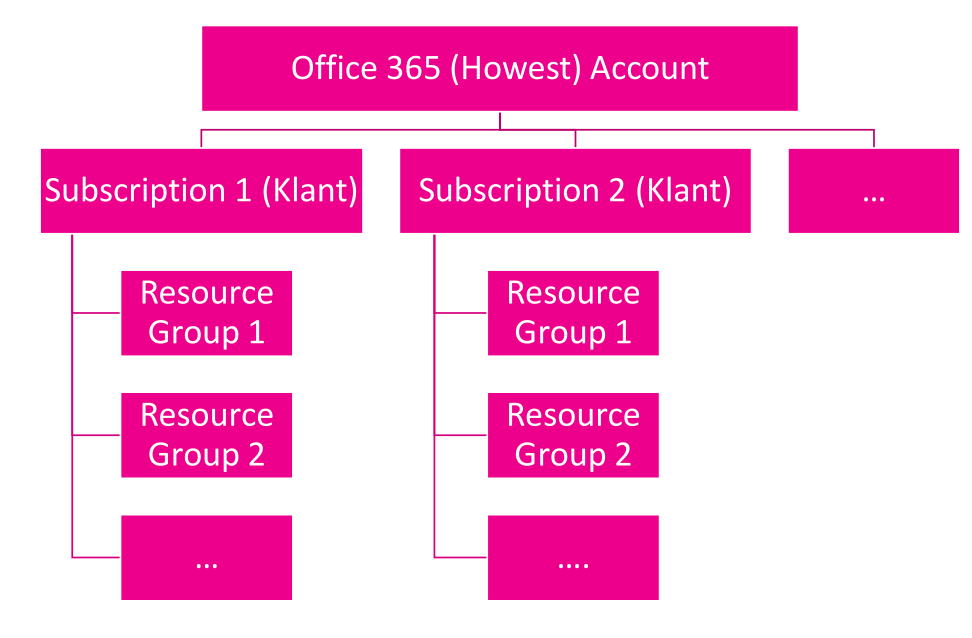
\includegraphics[width=0.5\textwidth]{resource-group.png}
    \caption{Resource groups}
\end{figure}

\begin{itemize}
    \item Logische container
    \item Per project
    \item Per soort services
    \begin{itemize}
        \item Storage
        \item Webservers
        \item Fileservers
        \item SQL, Blob, \dots
    \end{itemize}
    \item Je kiest dit zelf
    \item Makkelijk om te testen, je kan een volledige container verwijderen zonder dat je alles apart moet verwijderen
    \item Toegangsrechten per container zijn mogelijk
    \begin{itemize}
        \item via Office 365 account
    \end{itemize}
    \item Je kies datacenter locatie van je resource group, niet alle resources moeten op dezelfde locatie staan als je resource group.
\end{itemize}

\subsection{Azure Virtual Machines}
\begin{itemize}
    \item Eigen server op Azure omgeving
    \item Meestal on-premise (server op bedrijf) die we virtueel verplaatsen naar Azure
    \item Heel wat mogelijkheden
    \begin{itemize}
        \item File servers
        \item Database servers
        \item Webservers
        \item Application servers
        \item ...
    \end{itemize}
    \item Toegang tot resources op server die niet mogelijk zijn via een web applicatie
    \begin{itemize}
        \item Bv. communicatie met oude software pakketten
        \item Bv. Genereren van Word/Excel documenten
        \item \dots
    \end{itemize}
\end{itemize}

\subsubsection{Waarom?}
Wanneer je volledige controle wenst over je machine

\begin{itemize}
    \item Volledige controle == volledige verantwoordelijkheid!
    \begin{itemize}
        \item Niet te onderschatten
        \item Security, patching, scaling
    \end{itemize}
    \item Windows
    \item Linux
\end{itemize}

\subsubsection{Maintenance}

\begin{itemize}
    \item Planned maintenance
    \begin{itemize}
        \item Updates van het Azure platform (stabiliteit, security, performance)
        \item Soms moet de VM herstarten
    \end{itemize}
    \item Unplanned maintenance
    \begin{itemize}
        \item Storing in de onderliggende architectuur (netwerk-, disk-, rack-problemen)
        \item Azure zal automatisch VM verplaatsen naar werkende infrastructuur
    \end{itemize}
\end{itemize}

Hoe kan ik mijn VM `up and running' houden?
\begin{itemize}
    \item Availability set
    \begin{itemize}
        \item Garantie van 99.95\% uptime
        \item Minstens 2 virtual machines nodig
        \item Duurder
    \end{itemize}
\end{itemize}

\subsection{Azure Web App}
\begin{itemize}
    \item Azure Platform Service
    \item Laat ons toe om webapps online te plaatsen
    \item We moeten GEEN eigen server aanmaken
    \item We moeten GEEN webserver configureren
    \item Click \& go
    \item Ondersteuning voor:
    \begin{itemize}
        \item ASP.NET (Core)
        \item PHP
        \item Python Flask
        \item Java
        \item Node.JS
        \item \dots
    \end{itemize}
    \item Makkelijkste manier om uw applicatie online te krijgen, easy deployment
    \item Eenvoudige te koppelen aan een GitHub Repository
    \item Autoscale (not free)
    \item Monitoring
    \item Staging mode
\end{itemize}

\subsubsection{Free}
= gratis plan voor Azure Web App

\begin{itemize}
    \item Gedeelde server met andere web apps
    \item Je weet niet welke server, is transparant voor gebruiker
    \item 1GB storage
    \item Beperking op trafiek per dag: 165MB
\end{itemize}

\subsubsection{Shared}
\begin{itemize}
    \item Gedeelde server
    \item 1GB storage
    \item Mogelijkheid tot DNS vb: www.mijnnaam.be
\end{itemize}

\subsubsection{Basic, Premium}
\begin{itemize}
    \item App service plan $\Rightarrow$ eigen server, dus niks delen met derden (je kan niet inloggen op die server)
    \item SSL
    \item Custom domains
    \item CPU keuze
    \item Memory keuze
    \item Scaling tot 3 toestellen
\end{itemize}

\subsection{Scaling}

\subsubsection{Scale Up}
\begin{itemize}
    \item = vertical scaling
    \item Server krachtiger maken, meer memory en CPU
\end{itemize}

Pros: 
\begin{itemize}
    \item Minder energie dan scale out
    \item Eenvoudiger te implementeren
    \item Minder licenties (n.v.t. op Azure Web App)
\end{itemize}

Cons:

\begin{itemize}
    \item Duurder
    \item Indien we maar 1 machine gebruiken: $\Rightarrow$ hardware failure en toepassing is down
\end{itemize}


\subsubsection{Scale Out}
\begin{itemize}
    \item = horizontal scaling
    \item Meerdere machiens maar minder krachtig
\end{itemize}

Pros: 
\begin{itemize}
    \item Goedkoper
    \item Betere bescherming bij hardware failure, hebt meerdere machines
\end{itemize}

Cons:

\begin{itemize}
    \item Meer licenties nodig (n.v.t. op Azure)
    \item Meer plaats in datacenter
    \item Meer energieverbruik
    \item Complexer netwerk
    \item Soms toepassing aanpassen
\end{itemize}

\subsection{Azure SQL}

\begin{itemize}
    \item 
    \item SQL Server Database op Cloud platform
    \item We moeten zelf geen hardware/software aankopen
    \item Niet verantwoordelijk voor backups
    \item Eenvoudige schalen bij zware loads
    \item 3 opties
    \begin{itemize}
        \item Serverless Managed Database (onze voorkeur)
        \item SQL Managed Instance
        \item SQL Virtual Machine
    \end{itemize}
\end{itemize}

\subsubsection{SQL Server Cloud Based}
\begin{itemize}
    \item Compatible met SQL server 2012
    \item Te beheren via Enterprise manager
    \item Werkt zoals een gewone SQL server
    \item Connecteren is mogelijk via:
    \begin{itemize}
        \item .NET
        \item Python
        \item PHP
        \item Node
        \item \dots
    \end{itemize}
    \item High Availability
    \begin{itemize}
        \item Replicatie over 3 servers (default)
        \item Automatische Back-ups
    \end{itemize}
    \item Database draait op een server
    \item Verschillende pricing mogelijkheden
\end{itemize}

\subsubsection{Eigenschappen}
\begin{itemize}
    \item Database draait op een server
    \item Verschillende pricing mogelijkheden
\end{itemize}

\subsubsection{Security}
Azure FireWall: IP adres van je netwerk toelaten

\subsubsection{Azure DTU}
\begin{itemize}
    \item DTU = Database Transaction Units
    \item Soort `munteenheid'
    \item Gemengde eenheid van:
    \begin{itemize}
        \item CPU
        \item Memory
        \item I/O
    \end{itemize}
    \item Deze resources krijg je ter beschikking
    \item Hoe meer DTU, hoe meer power, hoe duurder
    \item \url{https://docs.microsoft.com/en-us/azure/sql-database/sql-database-what-is-a-dtu}
    \item vCores = virtuele CPUs die de service mag gebruiken
\end{itemize}

\subsubsection{Throttling}
= Onderbreken van database communicatie omdat je teveel resources (DTU's) gebruikt (zelf voor retry zorgen).

\begin{figure}[H]
    \centering
    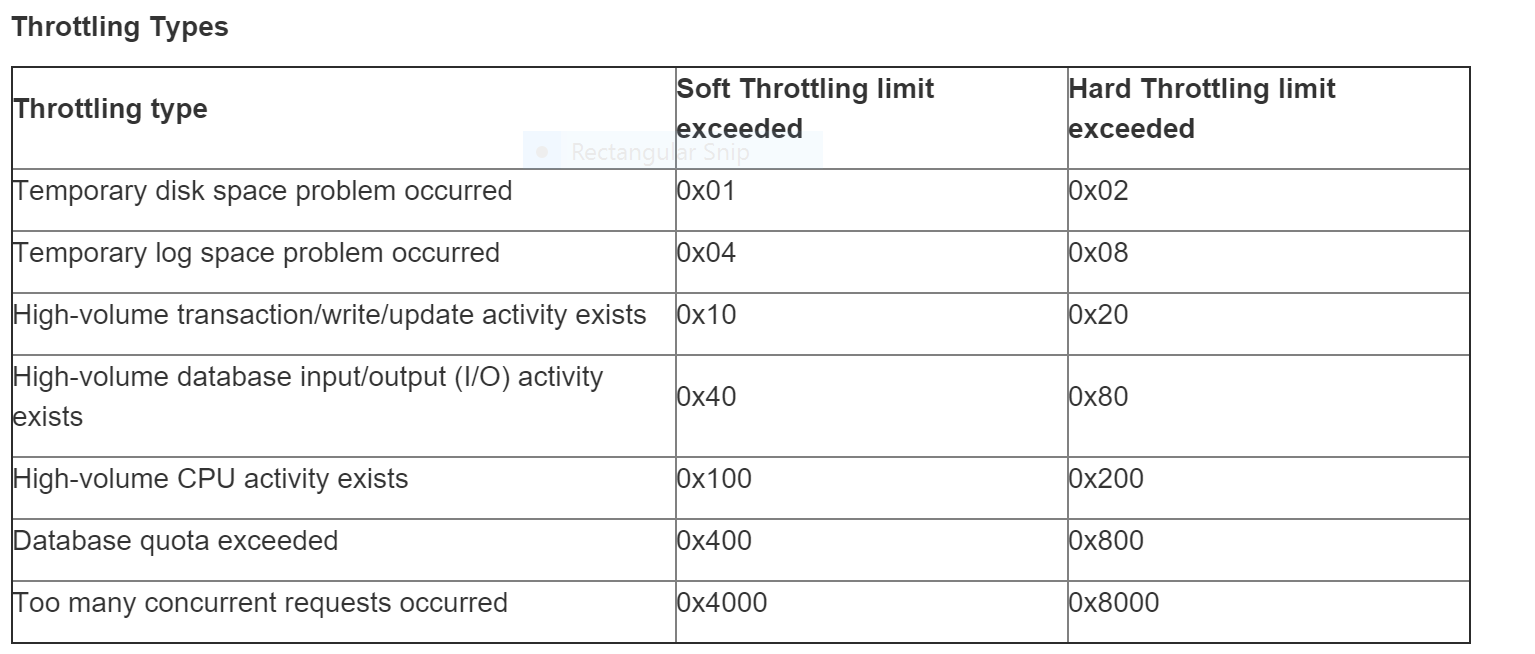
\includegraphics[width=0.8\textwidth]{azure-throttling.png}
    \caption{Throttling types}
\end{figure}

\begin{figure}[H]
    \centering
    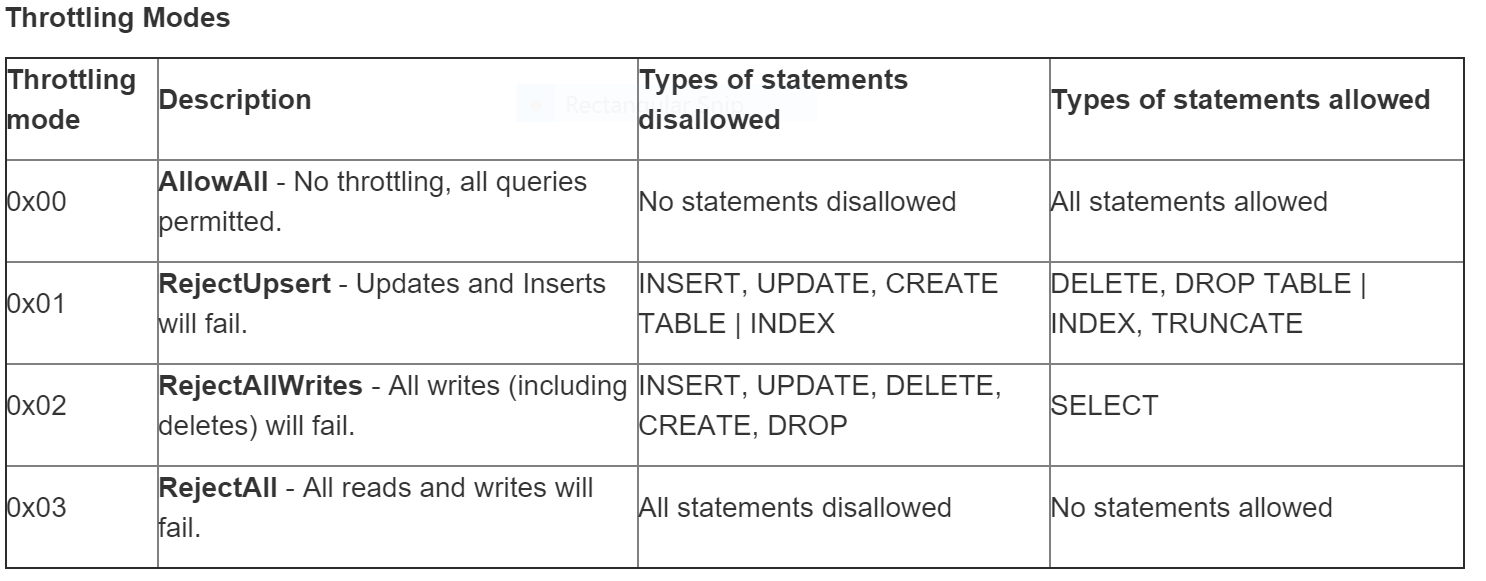
\includegraphics[width=0.8\textwidth]{azure-throttling-modes.png}
    \caption{Throttling modes}
\end{figure}

\begin{figure}[H]
    \centering
    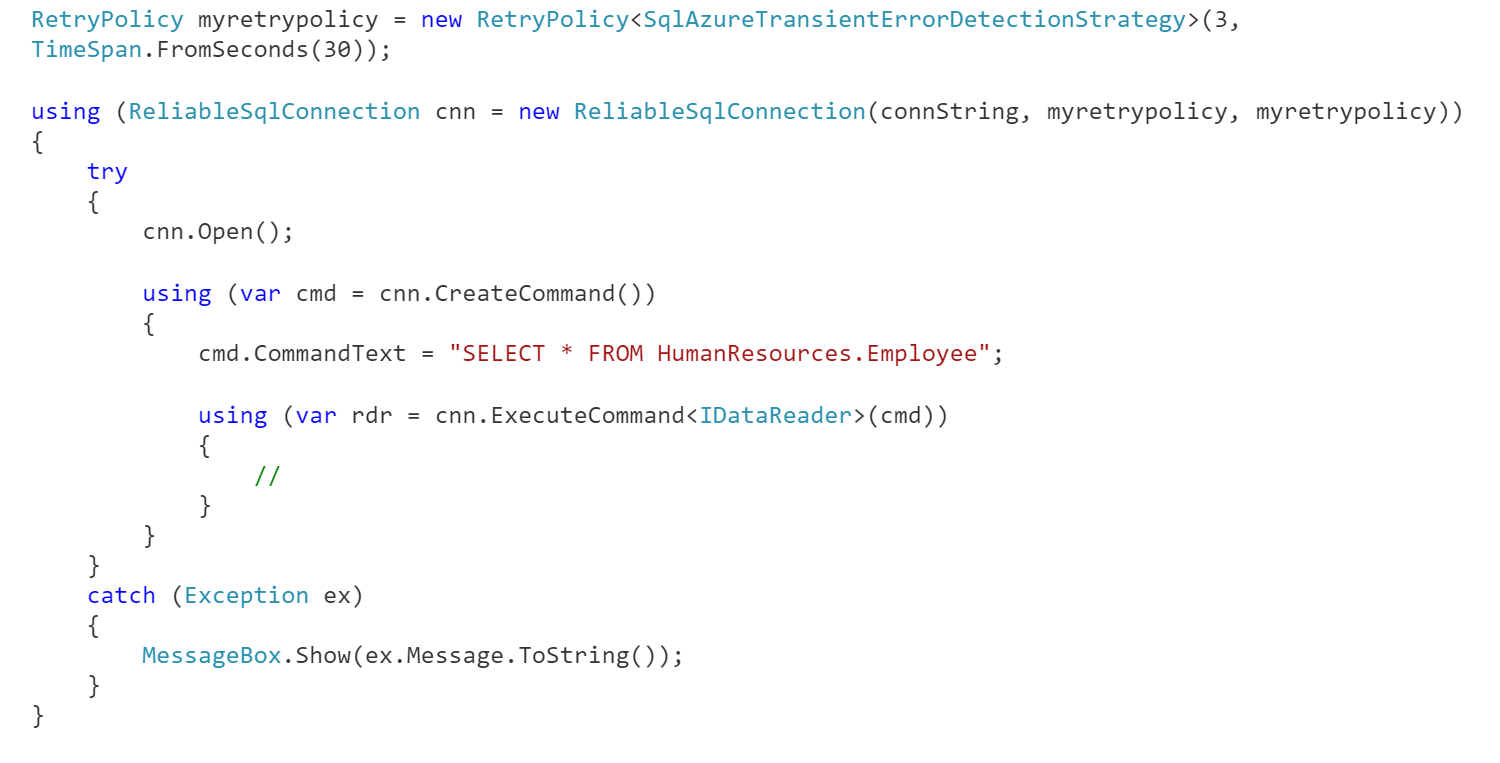
\includegraphics[width=0.8\textwidth]{azure-sql-command-ex.png}
    \caption{Voorbeeld SQL command in C\#}
\end{figure}


\subsubsection{Resources}
\begin{itemize}
    \item \url{https://msdn.microsoft.com/en-us/library/azure/dn338079.aspx}
    \item \url{http://geekswithblogs.net/ScottKlein/archive/2012/01/27/understanding-sql-azure-throttling-and-implementing-retry-logic.aspx}
\end{itemize}

\subsubsection{Azure Database for MySQL}

\begin{itemize}
    \item Toegang via MySQL Workbench
    \item Werkt zoals een gewone MySQL DB
    \item Je moet geen eigen servers opzetten, is volledig managed
    \item Automatische Back-ups
\end{itemize}

\subsection{Azure \& Internet of Things}

\subsubsection{Waarom is Azure belangrijk voor IoT?}

\begin{itemize}
    \item Azure Event Hubs
    \begin{itemize}
        \item Ontvangen van berichten afkomstig van toestellen
    \end{itemize}
    \item \textcolor{red}{Azure IoT Hub}
    \begin{itemize}
        \item Ontvangen van berichten
        \item Versturen van berichten naar toestellen
    \end{itemize}
    \item Azure Streaming Analytics
    \begin{itemize}
        \item Verwerken van events afkomstig van Event Hubs en IoT Hub
    \end{itemize}
\end{itemize}

\bold{Bovenstaande zeer belangrijk voor ons!}

\begin{figure}[H]
    \centering
    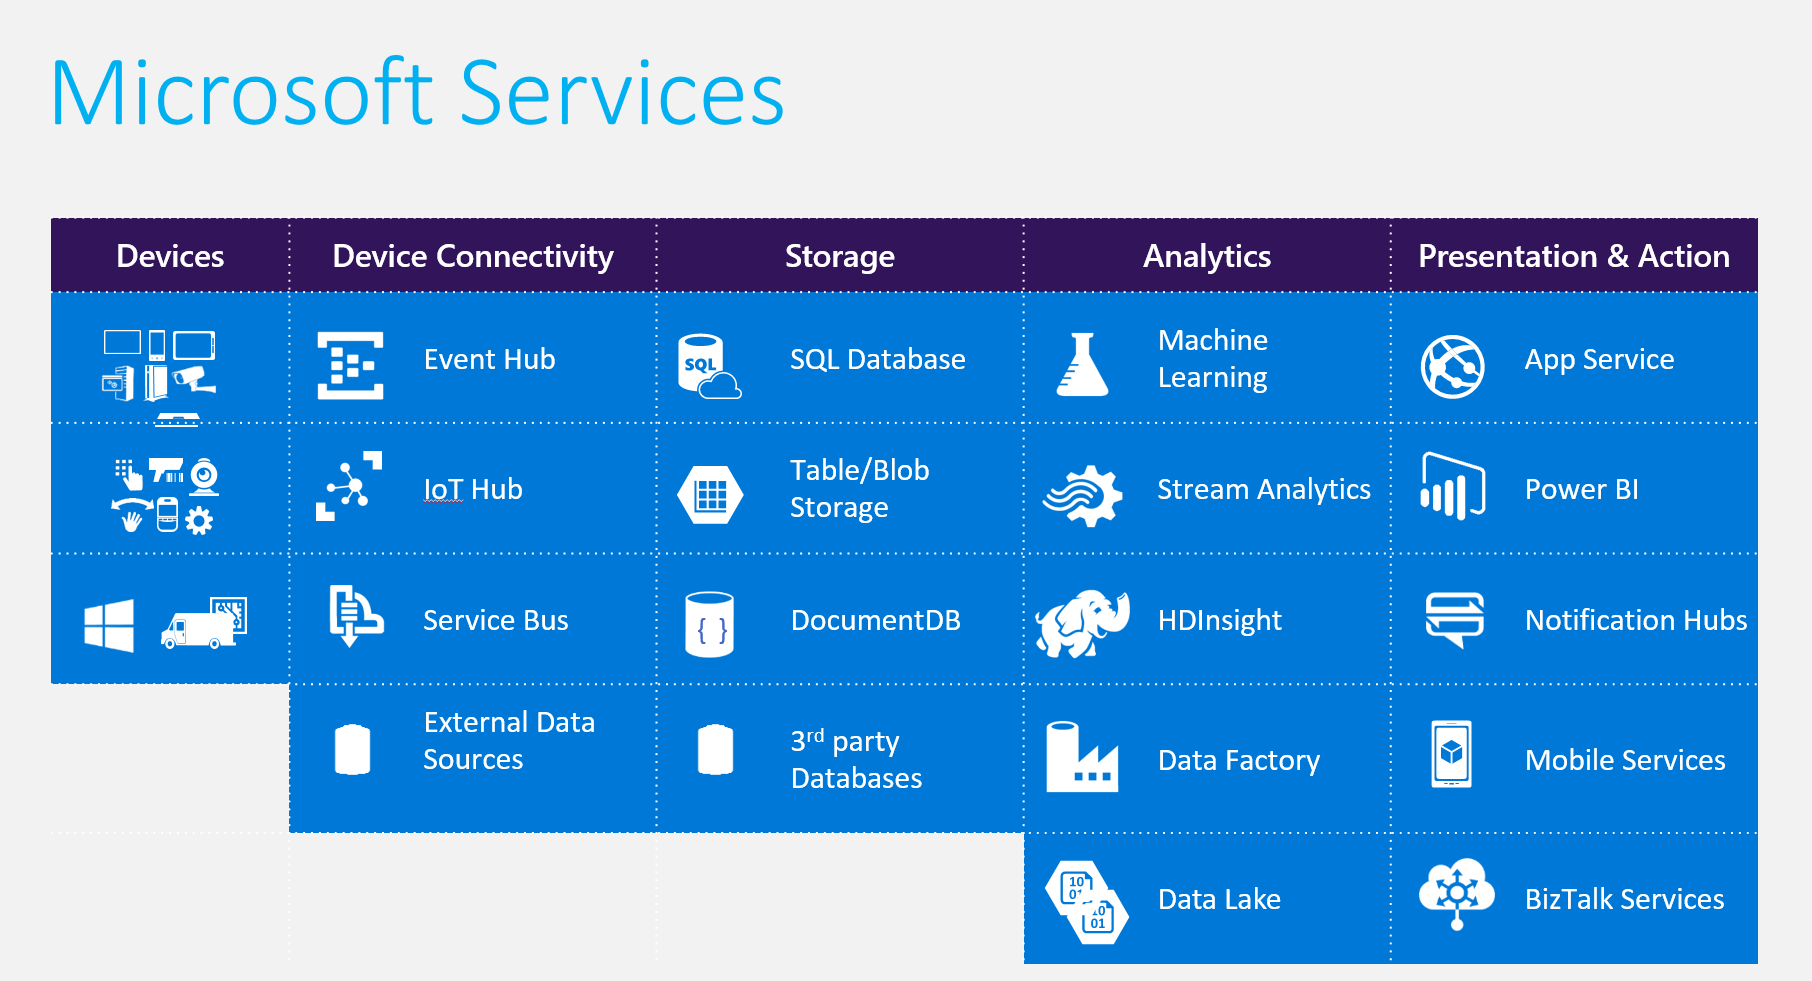
\includegraphics[width=0.8\textwidth]{azure-iot-microsoft-services.png}
    \caption{Microsoft Services}
\end{figure}

\subsection{Azure CLI}

\subsubsection{Azure Portal}

\begin{itemize}
    \item OK voor dagelijks gebruik
    \item Niet makkelijk te automatiseren
    \item Wat als ik 100 sites nodig heb?
    \item Wat als ik 50 servers nodig heb?
\end{itemize}

\subsubsection{Oplossing: Azure CLI 2.0}
\begin{itemize}
    \item Commandline Azure resources aanmaken
    \item Makkelijk met scripts
    \item Ideaal voor DevOps
\end{itemize}

\subsection{Bash/Powershell}

\begin{itemize}
    \item Bash commandline in portal
    \item Alles wat je via UI kan doen kan je ook via commandline in de portal
\end{itemize}

\subsection{Andere Azure onderdelen}
\begin{figure}[H]
    \centering
    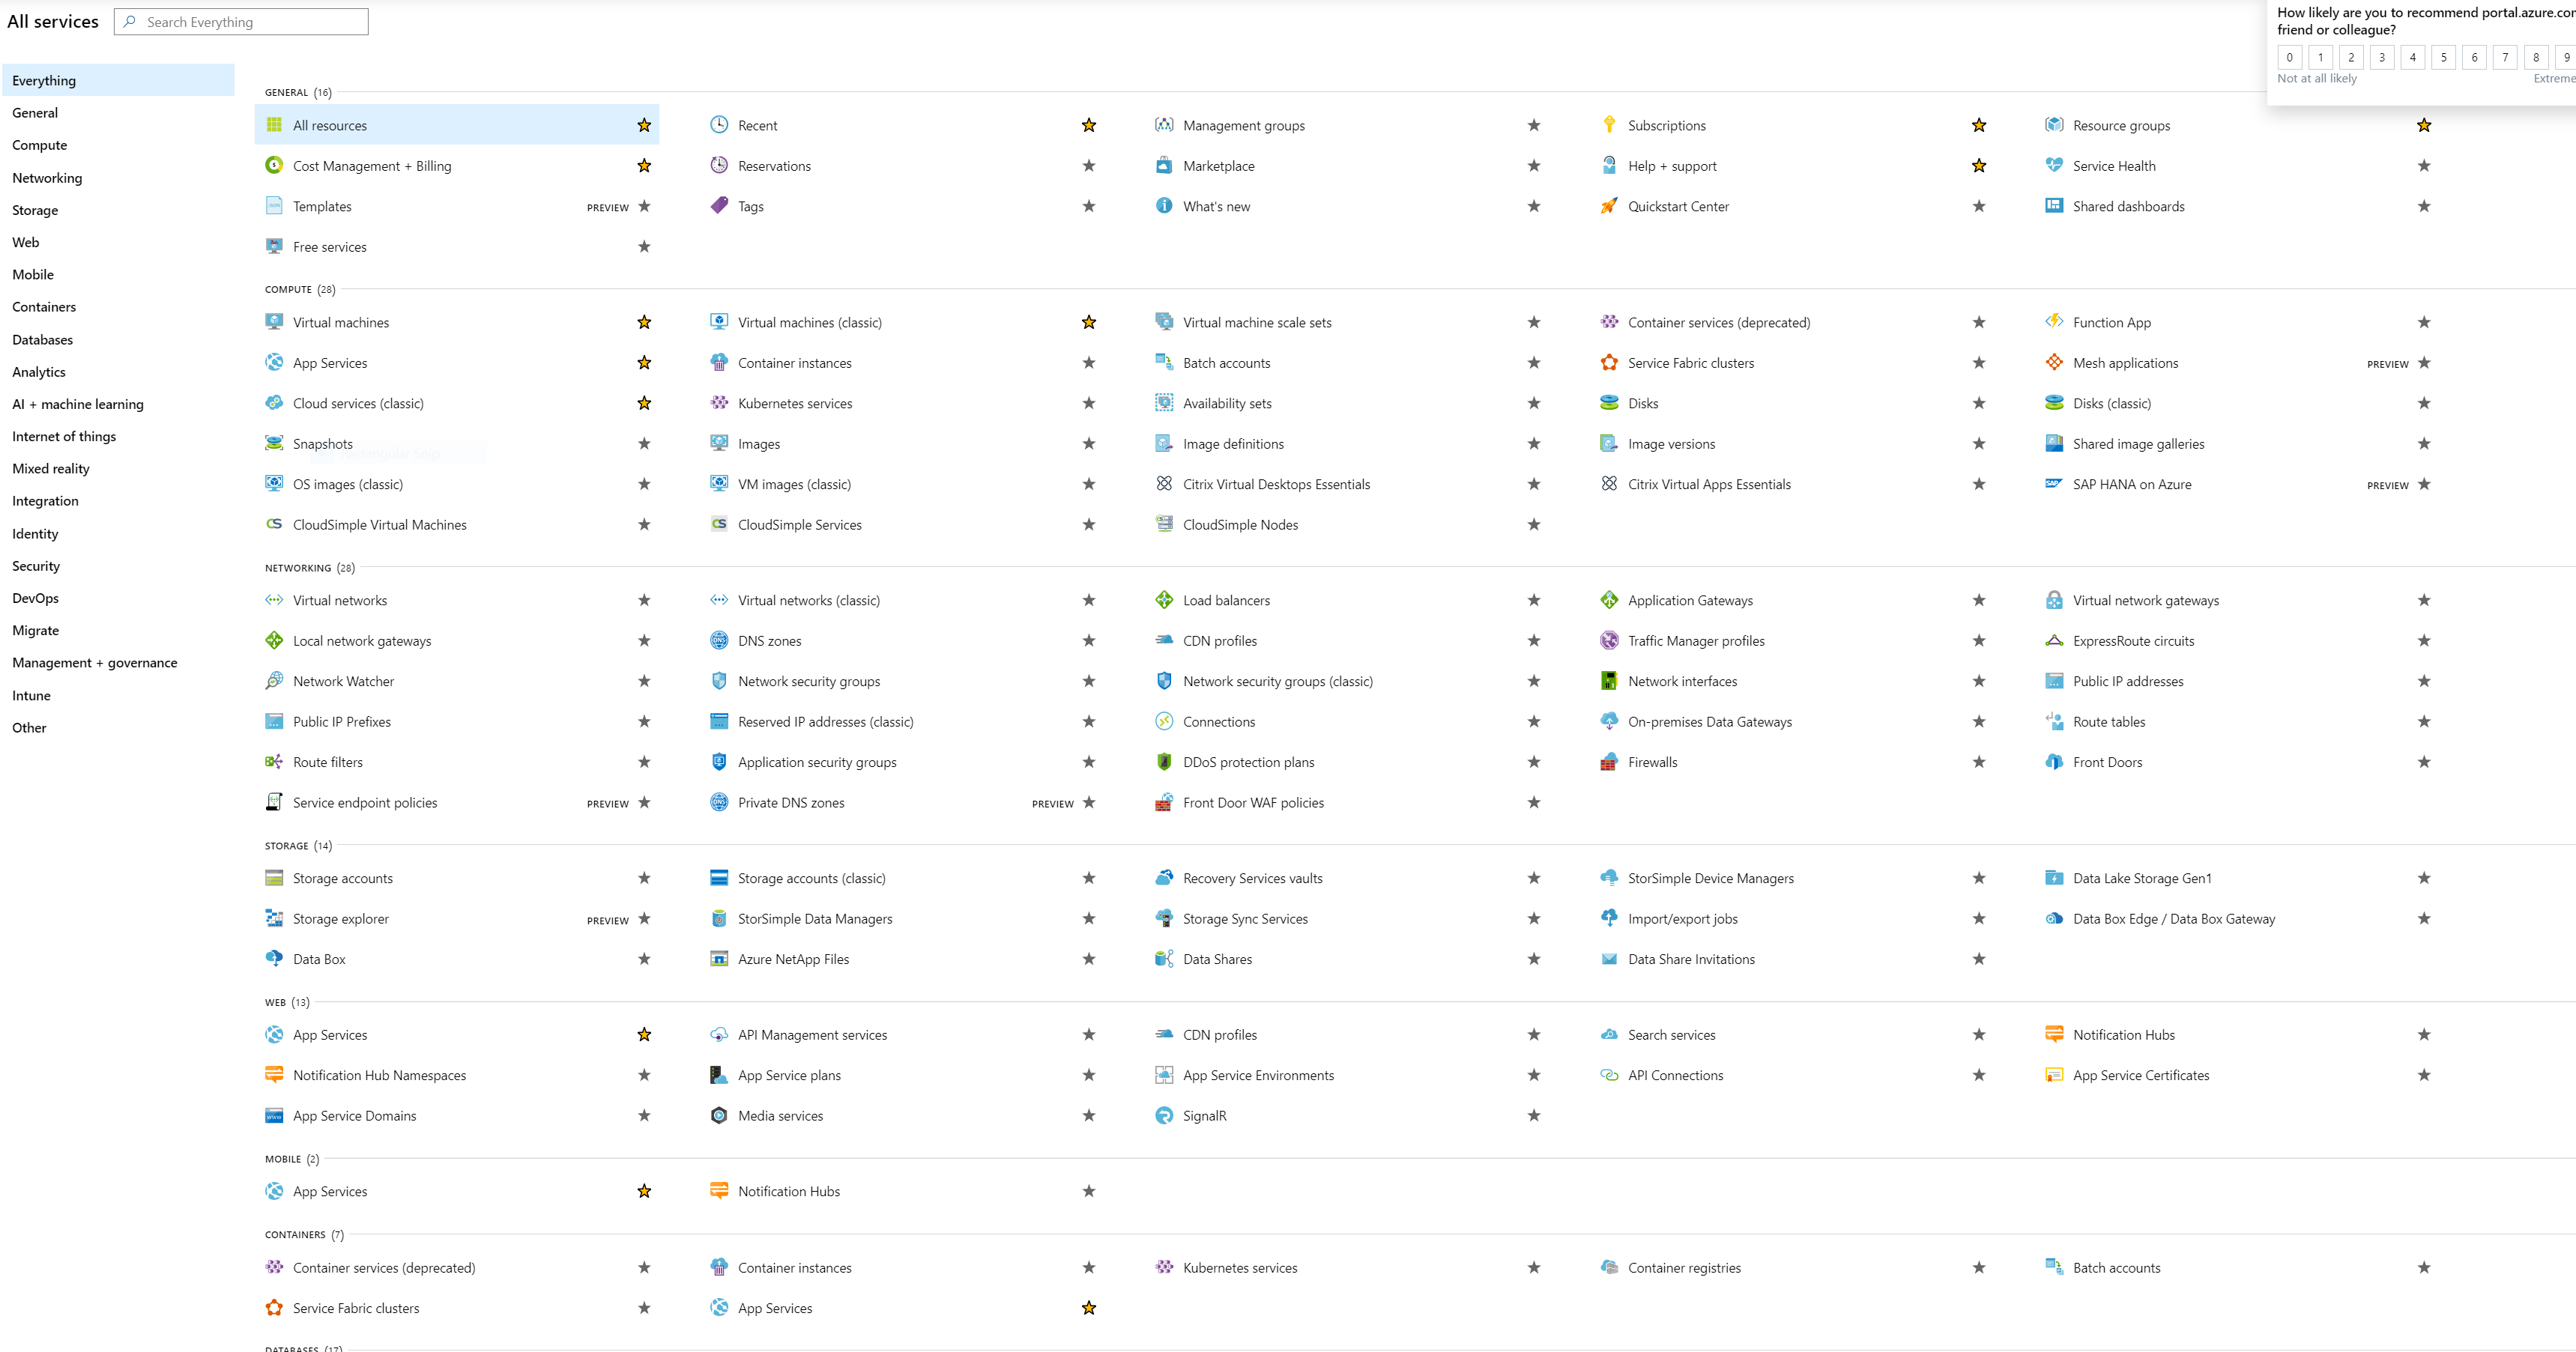
\includegraphics[width=0.95\textwidth]{azure-onderdelen.png}
    \caption{}
\end{figure}

\subsection{Samenvatting}
\begin{itemize}
    \item Wat is Cloud computing?
    \item Wie zijn de grote spelers?
    \item Welke soorten zijn er en wat zijn hun eigenschappen?
    \item Wat is een Azure subscription?
    \item Wat zijn resource groups?
    \item Hoe kan je scalen?
    \item Voor en nadelen van Azure VM’s?
    \item Wanneer Azure VM gebruiken?
    \item Wat is SQL Azure en wat zijn DTU’s?
    \item Wat is throttling?
    \item Wat is een Azure Web App?
\end{itemize}


\section{Examen}
\begin{itemize}
    \item Theorie: 30\%
    \item Labo 70\%
    \item Het examen bevat zeker vragen over ofwel MQTT ofwel IoT
\end{itemize}

\end{document}